\chapter{Background}
In this section, the background of the most important technologies used will be presented, setting up grounds for discussion.

\section{Artificial Intelligence}

IBM defines Artificial Intelligence as the use of technology to enable computers and machines to replicate human intelligence and problem-solving abilities.

Artificial intelligence (AI), whether used independently or combined with other technologies like sensors and robotics, accomplishes tasks that are typically performed by humans. Examples include digital assistants, GPS navigation, autonomous vehicles, and sophisticated AI tools like OpenAI's ChatGPT, which are widely used in today's society.

In the field of computer science, AI includes areas like machine learning and deep learning, which aim to mimic human thinking through algorithmic systems. These algorithms can "learn" from the data they receive, getting better at making decisions over time through continuous improvement processes.


Artificial intelligence can be categorized into two groups: Weak AI and Strong AI.

Weak AI, also called narrow AI or artificial narrow intelligence (ANI), is designed and trained for specific tasks, driving much of today's AI applications like Siri, Alexa, IBM Watson, and self-driving cars. On the other hand, strong AI consists of artificial general intelligence (AGI) and artificial super intelligence (ASI). AGI aims to match human intelligence, possessing self-awareness and problem-solving abilities, while ASI would surpass human intelligence. Although strong AI remains theoretical, ongoing research explores its potential \cite{IBM}. 

\subsection{Natural Language Processing}

Natural Language Processing (NLP) refers to a set of computational techniques designed for automatically analyzing and representing human languages. It involves tasks such as accessing and acquiring lexical, semantic, and episodic characteristics of language, creating and propagating dynamic bindings, manipulating recursive structures, coordinating processing modules, identifying language constructs, and representing abstract concepts. The ultimate goal of NLP is to advance from basic language processing to achieving natural language understanding, which involves grasping context and meaning beyond mere syntactic structures. Presently, NLP heavily relies on syntactic representations, which are constrained by their inability to incorporate background knowledge similar to human comprehension. The focus of NLP centers on replicating human cognitive processes and leveraging semantic features that are implicit in the text. These computational models support both theoretical exploration and practical implementations, enabling efficient communication between humans and machines \cite{Chowdhary2020}.

\subsection{Transformers}
Transformer architectures leverage a self-attention mechanism to understand relationships within sequences, allowing them to capture long-range dependencies more effectively compared to recurrent networks. Unlike traditional models that rely on recursion, Transformers process entire sequences at once, improving scalability and efficiency. They are built solely on attention mechanisms, with a unique implementation known as multi-head attention, optimized for parallelization. Transformers excel in handling complex models and large datasets, offering advantages over alternatives like hard attention, which relies on stochastic sampling. Due to their minimal prior knowledge assumption, Transformers are typically pre-trained on large-scale unlabeled datasets using pretext tasks, enabling them to encode rich and generalizable representations. These representations are then fine-tuned on supervised tasks to achieve optimal performance \cite{KhanNHZKS}.

\subsection{Generative and Conversational AI}

Generative AI is a type of Artificial Intelligence that uses deep learning models to create human-like content in response to complex prompts, such as languages, instructions, or questions. Examples of this technology include OpenAI’s ChatGPT \cite{ChatGPT} and DALL-E \cite{DallE}. These AI models generate responses that go beyond their explicit programming, distinguishing them from other AI models. Conversational AI is an Artificial Intelligence subset that focuses on human-like interactions, often relying on predefined responses. However, some Conversational AI models can also generate content. Models like ChatGPT use both Generative and Conversational AI to enhance their capabilities, allowing them to better simulate human conversation and generate more dynamic responses. \cite{LimGPPP}

\subsubsection{ChatGPT}
ChatGPT, an AI-driven service accessible online, is designed for tasks such as text organization, summarization, and composition. GPT, short for "Generative Pre-trained Transformer", describes the manner in which ChatGPT processes requests and generates responses. It is built to understand and respond to user queries and commands by analyzing extensive text data to grasp word relationships. By predicting the most probable next word, similar to search engine auto-complete features, ChatGPT refines its responses iteratively. During training, exemplified by completing sentences such as "instead of turning left, she turned ...", ChatGPT evolves from random word suggestions to more accurate predictions. Because of the wide variety of possible answers, the model's numerical settings, called "weights" or "parameters," slowly change as it learns, capturing what it learns without saving or copying the original sentences \cite{OpenAICGPT}.

In response to natural language inputs, also called "prompts", ChatGPT provides text output. One example of such a prompt would be: "Explain to me in one paragraph what ChatGPT is." ChatGPT provided the following answer (Fig \ref{ChatGPT}).

\textit{
	ChatGPT is an advanced language model developed by OpenAI that uses deep learning techniques to generate human-like text responses. Trained on a vast amount of internet text, it has the ability to understand and generate coherent and contextually relevant responses to user queries, making it a powerful tool for conversational interactions, information retrieval, and providing assistance across a wide range of topics.} \cite{OpenAI} 

\begin{figure}[ht!]
	\centering
	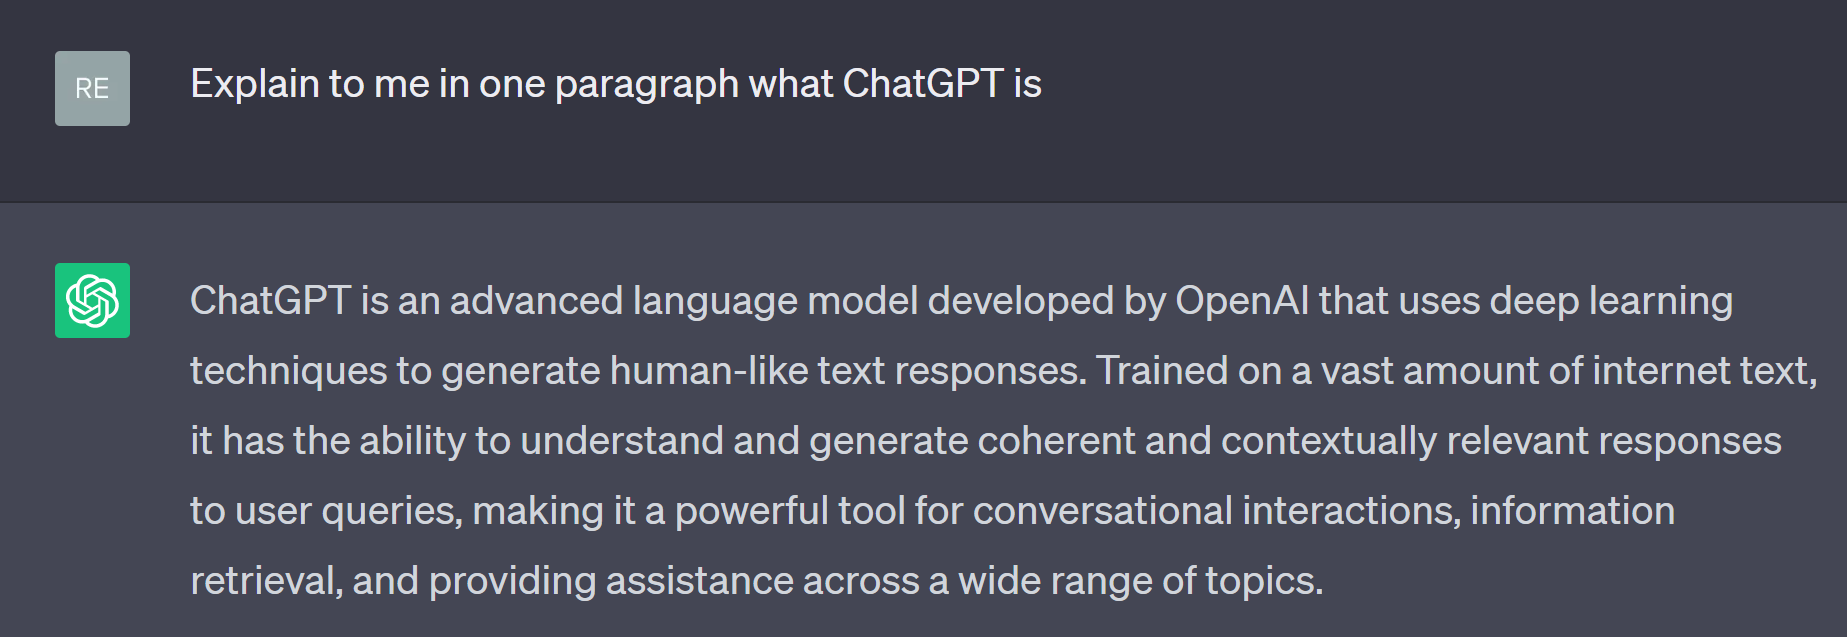
\includegraphics[width=90mm]{images/ChatGPT.png}
	\caption{ChatGPT - prompt and answer \label{ChatGPT}}
\end{figure}



\subsubsection{Prompt Engineering}
\label{prompt engineering}
Prompt engineering is the process of using prompts to program Large Language.
Models (LLMs), like ChatGPT. An LLM is given a set of instructions called a prompt
to help it tailor its output and user interactions. Engineering prompts to enforce
rules, automate procedures, and guarantee particular output qualities and output
quantities, which is known as prompt engineering. It is an ever-more-important skill set
required to communicate with LLMs and can be used to address a variety of issues,
such as automating software development tasks when speaking with LLMs. \cite{WhiteFHSOGESS}

Microsoft outlined a set of best practices in their guide to prompt engineering.

\begin{itemize}
	\item \textbf{Be specific}: Provide clear and precise instructions, minimizing room for interpretation and narrowing the operational scope.
	
	\item \textbf{Be descriptive}: Use descriptive language and analogies to enhance understanding.
	
	\item \textbf{Double Down}: Reinforce key points by repeating instructions, both before and after presenting primary content, employing cues for better comprehension.
	
	\item \textbf{Order Matters}:  Consider the order of information presentation, as it can influence the model's output. Be mindful of whether instructions precede or follow content, and recognize the impact of recency bias in the order of few-shot examples.
	
	\item \textbf{Give the model an "out"}: Offer the model an alternative option or an "out" in case it struggles with the assigned task. For instance, suggest a default response like "not found" to help the model avoid generating inaccurate information.\cite{MicrosoftLearn}
	
\end{itemize}

\section{Autonomous Vehicles}
There are six levels of driving automation, ranging from no driving automation (Level 0) to full driving automation (Level 5). At Level 0, vehicles are entirely manually controlled, with no automation in the dynamic driving task. 

Level 1 involves a single automation feature, like cruise control or steering assistance, while the driver retains control over other driving tasks. At Level 2, the car takes control over steering, acceleration, and braking. However, it still requires supervision from a human driver, who must take control when necessary.

Level 3 marks conditional driving automation, in which vehicles have environmental detection capabilities and can make informed decisions. However, human supervision and intervention are still necessary.

Level 4 introduces high driving automation, allowing vehicles to intervene in the event of system failures. While these cars can operate in self-driving mode, their use is limited to specific areas.

Level 5 represents full driving automation, where vehicles no longer require human attention. These fully autonomous cars have the ability to operate without restrictions, mimicking the capabilities of experienced human drivers.

Autonomous vehicles are vehicles that operate on Level 5 of the driving automation levels, which means they do not require human interaction\cite{Synopsys}\cite{SAEMobilus}\cite{TWI}.



\section{Computer Simulation}
The Cambridge Dictionary defines a simulation as \textit{a model of a real activity, created for training purposes or to solve a problem} \cite{CambridgeSim}.

A computer simulation is a program that imitates the operations of a real-world system or process over time. This program, referred to as a computer simulation model, uses algorithms to calculate the system's states over a specified time period, effectively creating a numerical representation of the system's evolution. The simulation generates data that can be visualized, often in a manner resembling scientific instrument readings. Simulations are typically used when a model's mathematical equations are complex and cannot be solved analytically, necessitating step-by-step computational methods. It's worth noting that the term "computer simulation", in the narrowest sense, refers to a specific implementation of an algorithm on a particular digital computer using a specific language and compiler. Variations in these elements can result in different outcomes from the simulation \cite{Winsberg}.

\subsection{Beamng.tech}
BeamNG.tech is an adapted version of the simulation game BeamNG.drive, created for academic and industrial purposes. While sharing many similarities, BeamNG.tech extends its functionality to support driver training and advanced driver-assistance systems (ADAS). It utilizes a soft-body physics engine for vehicle simulation \cite{BeamNG}.

Soft-body physics, as implemented in BeamNG.drive, is a fundamental aspect of the game's physics model. Unlike traditional "Rigid Body" physics simulation found in most games, BeamNG.drive utilizes a "Soft Body" physics simulation, which means that objects such as cars are deformable, allowing for more realistic and dynamic interactions \cite{BeamNGphysics}.

Additionally, BeamNG.tech incorporates tools such as BeamNGpy, a Python interface that automates testing and data gathering. Although its primary focus is on simulating ground-based vehicles, BeamNG.tech also offers simulations for air and maritime scenarios. Its research-oriented features include a sensor suite equipped with cameras, LIDAR, ultrasonic, electric, and IMU sensors tailored specifically for autonomous driving applications. BeamNGpy streamlines testing scenarios for learning systems and ensures the validation of autonomous driving software. While BeamNG.tech is not open-source, researchers can apply for a free license on their website \cite{BeamNG}.

\section{Procedural content generation}
In the realm of video games, procedural content generation (PCG) is the practice of using algorithms instead of manual design to generate elements like levels, characters, or environments. PCG has become increasingly significant in game development and technical game research because of its ability to efficiently create diverse and dynamic content. This approach involves the methodical application of algorithms and rules to produce content, providing developers with an automated and adaptable method to create a wide range of unique gaming experiences \cite{GambiMMFG}\cite{SummervilleSGHHINT}.

Procedural generation in the context of virtual roads involves generating roads by seamlessly connecting individual road segments. This approach ensures a continuous and gapless network, where each segment's front line serves as the back line for the subsequent one, resulting in a smooth transition. The procedural generation process also ensures that roads with impossible configurations are not created in order to maintain validity \cite{GambiMF}\cite{GambiMMFG}. 

\section {Testing of autonomous vehicles}

Testing is essential to make sure autonomous vehicles are safe, dependable, and compliant with the law. It helps to reduce risks and improve algorithms for making
decisions. Such testing increases public confidence in the technology by demonstrating safe and efficient functionality in a variety of driving scenarios.

\subsection{Field Testing}
Autonomous vehicles can be tested in real-world scenarios, like Google driverless cars, which are tested mainly in real traffic, according to Huang et al. \cite{HuangKYF}. Other real-world testing approaches include testing facilities. This form of testing is particularly beneficial because it mirrors the environment where the autonomous vehicle will eventually operate, providing a realistic assessment of its performance. 

While tests in real-world settings are always the final step in the validation chain, according to Huang et al., self-driving cars would have to drive hundreds of millions of kilometers without accidents to prove their safety statistically \cite{HuangKYF}. Since that is not feasible because of time and cost, simulation-based testing offers an alternative \cite{SchoenerHP}.

\subsection{Simulation-based testing}
The simulation-based testing of autonomous cars is carried out in a virtual setting, where the vehicles are evaluated against a variety of simulated scenarios that resemble real-world events. These scenarios can be repeated and altered as many times as necessary, incorporating different weather conditions, pedestrian movements, and traffic conditions. This allows the testing of uncommon or risky events without any real risk. Simulation testing is very valuable because it enables thorough testing in less time and at a lower cost than real-world testing. However, there are limitations since it depends on how accurately the simulations capture the complexity and unpredictability of real-world driving \cite{GambiMF}\cite{HuangKYF}\cite{PathrudkarMSC}.

\section{Context in Domain}
In the practical implementation, the prompts provided to ChatGPT will consist of high-level descriptions of roads. ChatGPT will generate more detailed descriptions of those roads as output. Subsequently, a Python program will translate these detailed road descriptions into nodes containing x, y, and z-coordinates. These translated road nodes will then be passed into the simulator using the BeamNGpy library. Within the simulator, a scenario will be constructed based on the road nodes received from the Python code, allowing for the visualization and simulation of the generated roads. By combining ChatGPT’s language generation capabilities, Python programming, and the simulation environment provided by BeamNG.tech, this system enables the generation, translation, and simulation of roads based on textual descriptions.